% =====================================================================
% fig-2-5-ligne-audit.tex  (corrigée)
% La ligne d'audit réelle écrite pour l'appel suivi en section 2.2.3 :
% première recherche de l'exécution 1 de S000 (journal mcp_audit.jsonl,
% 2026-09-11T11:35:58). Champs longs abrégés par .....
% Code couleur, aligné sur la légende de la figure :
%   bleu  = identifiant qui corrèle la session (run_id)
%   vert  = durée et version, qui datent la réponse
%   ocre  = arguments tronqués
%   rouge = résumé du résultat (jamais le résultat entier)
% Aucune bibliothèque TikZ particulière n'est requise.
% =====================================================================

\definecolor{auditbleu}{HTML}{1D5FA8}
\definecolor{auditvert}{HTML}{1F7A4D}
\definecolor{auditocre}{HTML}{B3541E}
\definecolor{auditrouge}{HTML}{B02A2A}
\definecolor{auditgris}{HTML}{4A5568}
\definecolor{auditfond}{HTML}{F7F7F4}

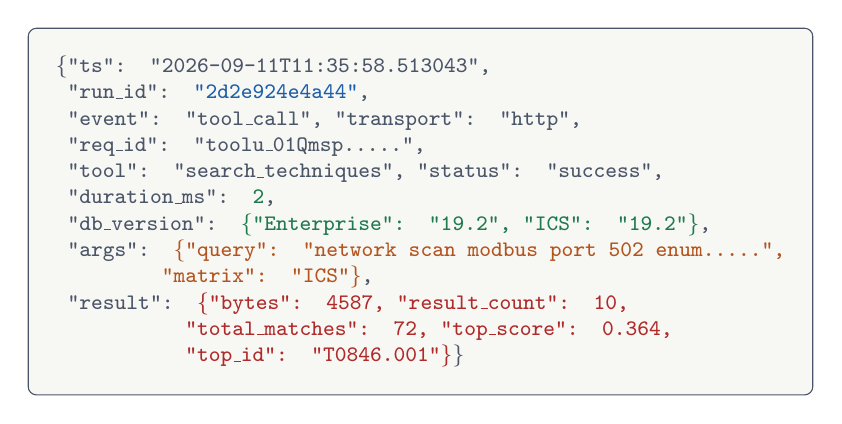
\begin{tikzpicture}
\node[draw=auditgris, fill=auditfond, rounded corners=3pt, inner sep=10pt,
      align=left, font=\ttfamily\footnotesize, text=auditgris]{%
\{"ts": "2026-09-11T11:35:58.513043",\\
\ "run\_id": \textcolor{auditbleu}{\textbf{"2d2e924e4a44"}},\\
\ "event": "tool\_call", "transport": "http",\\
\ "req\_id": "toolu\_01Qmsp.....",\\
\ "tool": "search\_techniques", "status": "success",\\
\ "duration\_ms": \textcolor{auditvert}{\textbf{2}},\\
\ "db\_version": \textcolor{auditvert}{\textbf{\{"Enterprise": "19.2", "ICS": "19.2"\}}},\\
\ "args": \textcolor{auditocre}{\textbf{\{"query": "network scan modbus port 502 enum.....",}}\\
\ \ \ \ \ \ \ \ \ \textcolor{auditocre}{\textbf{"matrix": "ICS"\}}},\\
\ "result": \textcolor{auditrouge}{\textbf{\{"bytes": 4587, "result\_count": 10,}}\\
\ \ \ \ \ \ \ \ \ \ \ \textcolor{auditrouge}{\textbf{"total\_matches": 72, "top\_score": 0.364,}}\\
\ \ \ \ \ \ \ \ \ \ \ \textcolor{auditrouge}{\textbf{"top\_id": "T0846.001"\}}}\}%
};
\end{tikzpicture}
